\documentclass[12pt]{article}
\usepackage[utf8]{inputenc}
\usepackage[T1]{fontenc}
\usepackage{lmodern}
\usepackage{graphicx}
\usepackage{subcaption}

\usepackage[svgnames]{xcolor}
\usepackage[a4paper,bindingoffset=0.2in,%
            left=0.5in,right=0.5in,top=0.5in,bottom=1in,%
            footskip=.25in]{geometry}
\pagenumbering{gobble}
\usepackage[colorlinks=true, linkcolor=Black, urlcolor=Blue]{hyperref}


\begin{document}
\title{Sprawozdanie - Odtwarzanie muzyki z nut na pięciolinii}
\author{Marcin Zatorski 136834, Sebastian Michoń 136770}
\date{\vspace{-2ex}}
\maketitle

\section{Cel i zakres projektu}
Celem projektu było zaimplementowanie aplikacji odczytującej nuty z obrazu z kamery, a następnie odtworzenie ich za pomocą głośnika z użyciem płytki Raspberry Pi.

\section{Schemat}
\begin{enumerate}
	\item \underline{Idea, połączenie, schemat - będą zdjęcia}
\end{enumerate}
	
\section{Projekt a realizacja}
Aplikacja została napisana w języku Python i Cython. Rozpoznawanie nut zostało zaimplementowane przy użyciu biblioteki OpenCV. Aplikacja jest w stanie rozpoznać nuty z wysoką skutecznością, o ile zdjęcie zostało zrobione w dobrych warunkach oświetleniowych. Algorytm rozpoznaje tylko część symboli - nuty (całe nuty, półnuty, ćwierćnuty i ósemki) oraz klucze. Tą część algorytmu można by rozszerzyć o rozpoznawanie większej ilości symboli. Dokładność rozpoznawania nut również można by ulepszyć na przykład poprzez zastosowanie maszynowego uczenia się.
	
W trakcie rozwijania projektu dużą przeszkodą była szybkość działania. Dzięki przepisaniu części kodu do języka Cython oraz optymalizacjom aplikacja działa zadowalająco szybko.
	
Pierwotnie w projekcie zakładaliśmy użycie płytki BeagleBone Black. Zdecydowaliśmy się jednak na użycie płytki Raspberry Pi - umożliwiło to proste podłączenie głośnika przez Bluetooth.
	
Aplikacja nie pozwala na wybranie dźwięku instrumentu, co było początkowo planowane. Aplikacja odtwarza jednocześnie nuty tylko z jednej pięciolinii, a nie z obu.
	
Aplikację można by rozwinąć o lepszy interfejs użytkownika. Obecnie aplikacja jest uruchamiana z linii poleceń. Warto by było dodać na przykład GUI pokazujące obraz z kamery lub przycisk umożliwiający wykonanie zdjęcia.

\section{Kluczowe fragmenty kodu}
\begin{enumerate}
	\item \underline{Które kody - integracja czy analiza nut? Dopiszę tu swoją część cythona, przynajmniej interfejsy}
	\item \underline{Pewnie także integracja z pythonem}
\end{enumerate}

\clearpage
\section{Zdjęcia fizycznych połączeń urządzeń}
\begin{figure}[h!]
	\centering
	\begin{subfigure}[b]{0.32\linewidth}
		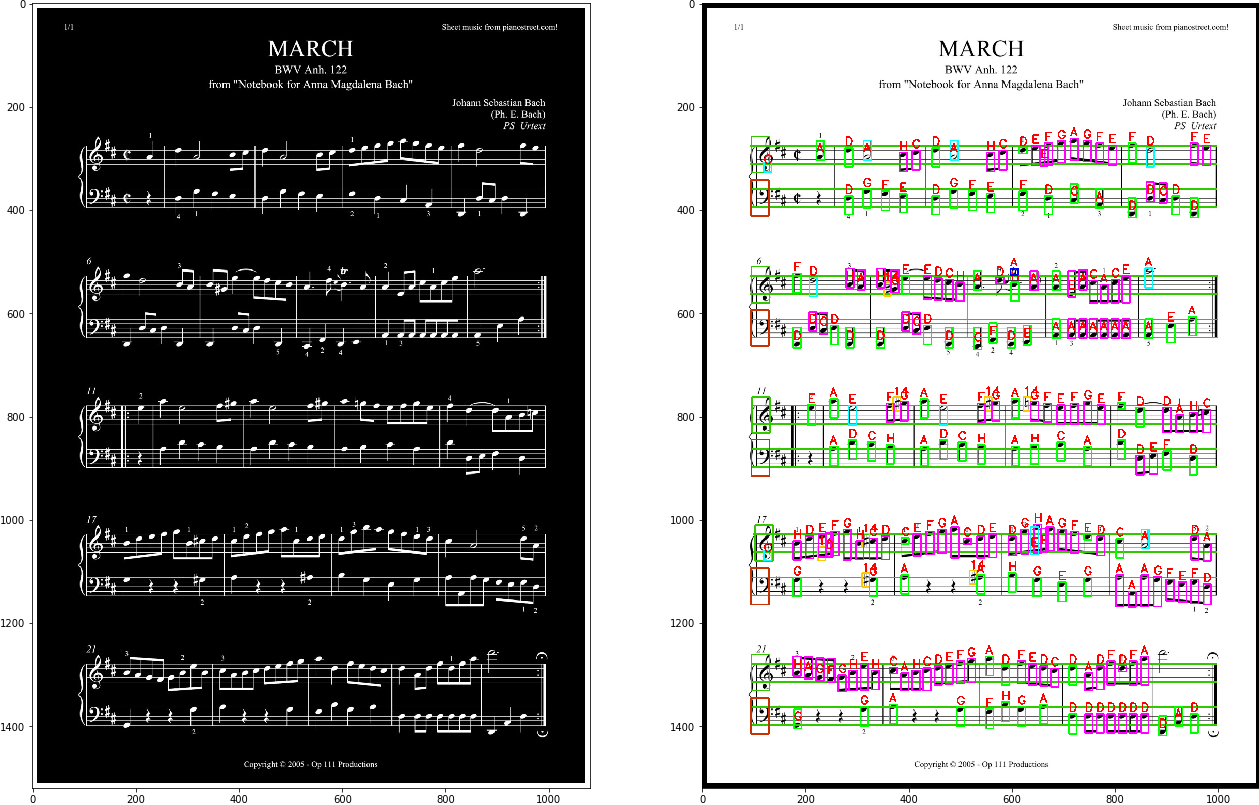
\includegraphics[width=\linewidth]{zdjs/Zdj0.png}
		\caption{Pierwszy podpis}
	\end{subfigure}
	\begin{subfigure}[b]{0.32\linewidth}
		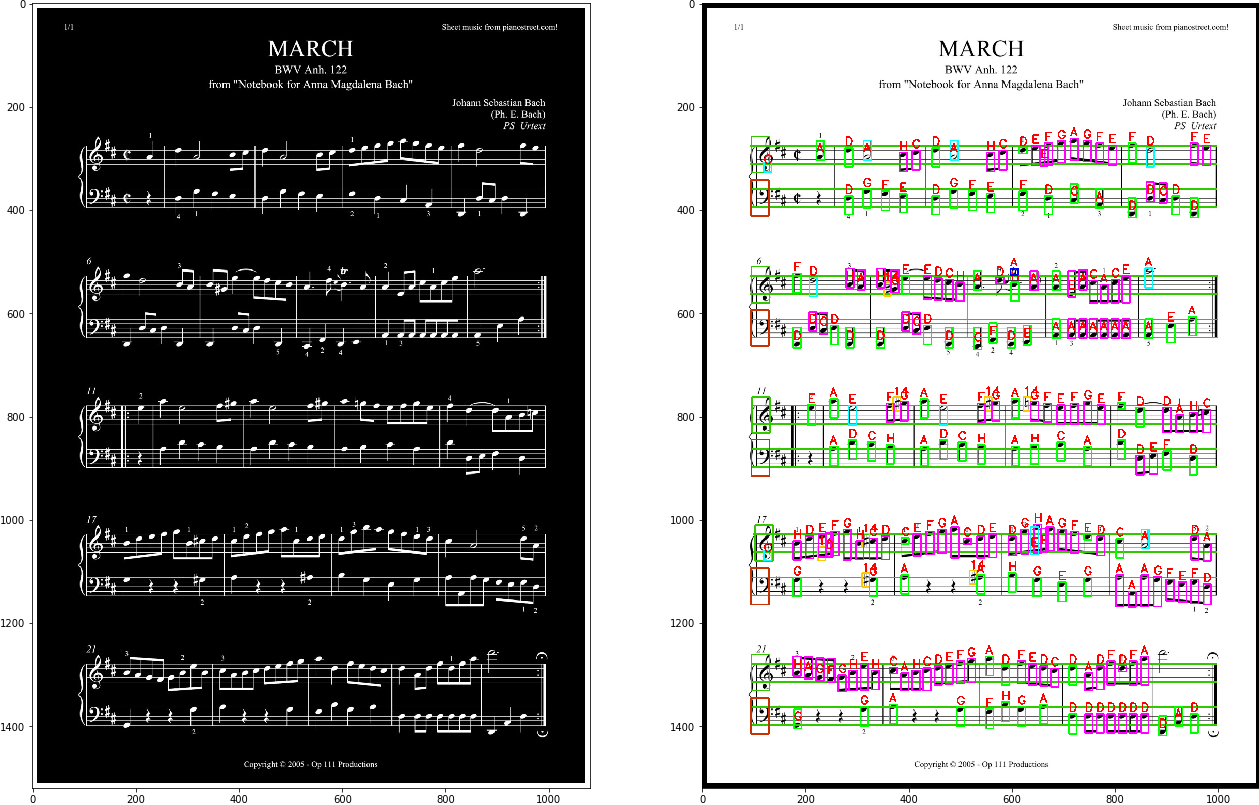
\includegraphics[width=\linewidth]{zdjs/Zdj0.png}
		\caption{Drugi podpis}
	\end{subfigure}
	\begin{subfigure}[b]{0.32\linewidth}
		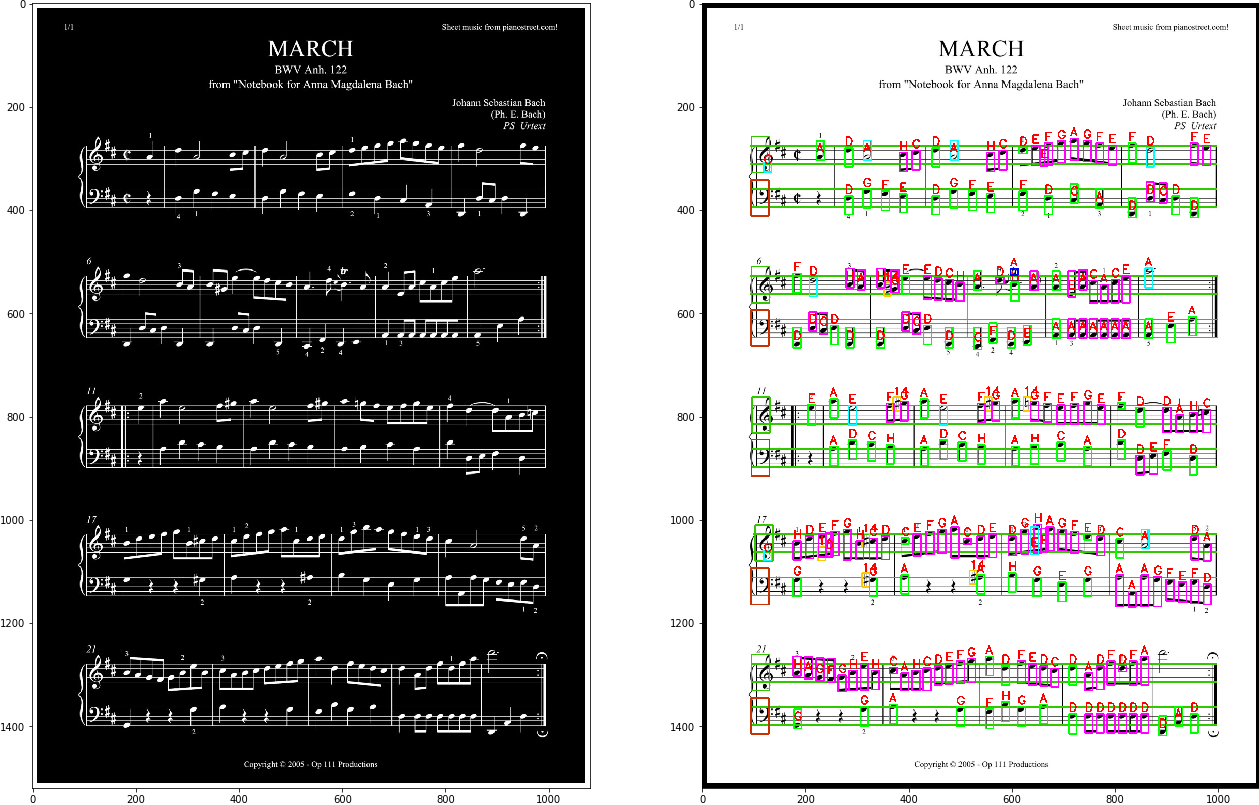
\includegraphics[width=\linewidth]{zdjs/Zdj0.png}
		\caption{Trzeci podpis}
	\end{subfigure}
	
	\begin{subfigure}[b]{0.48\linewidth}
		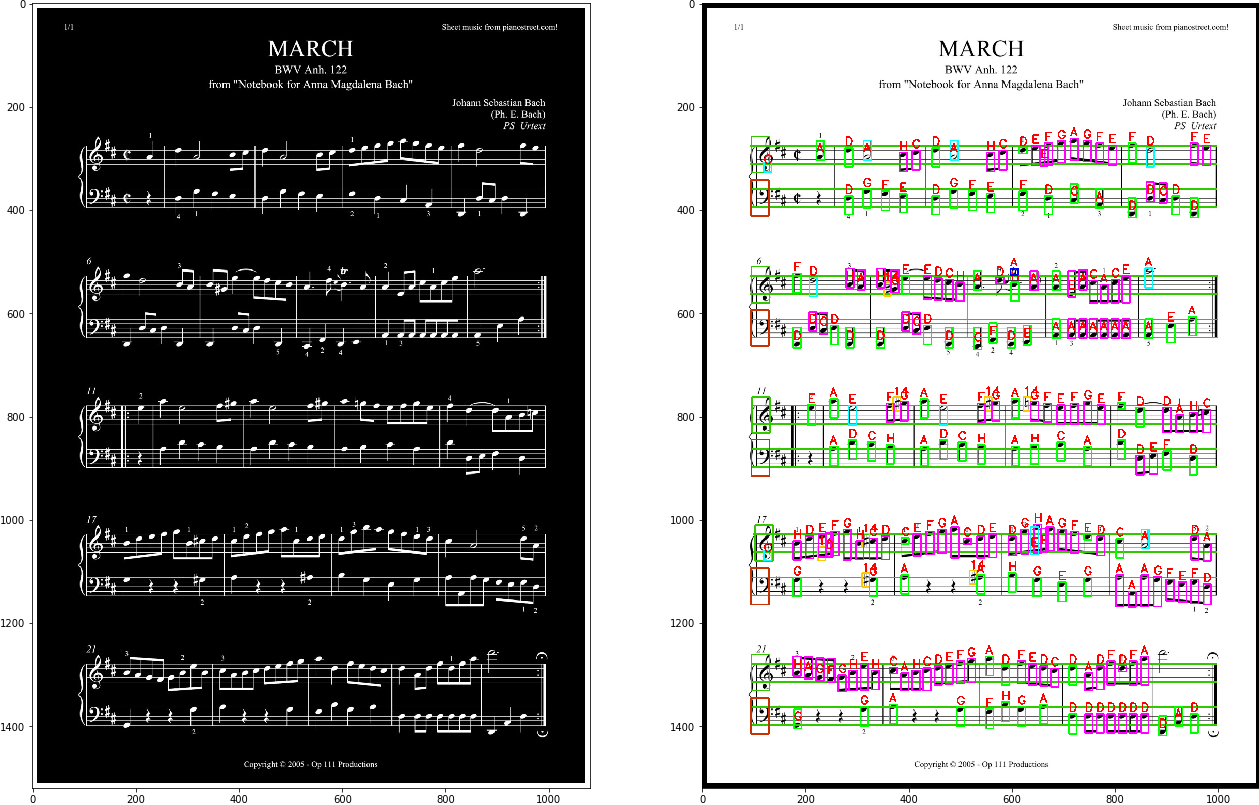
\includegraphics[width=\linewidth]{zdjs/Zdj0.png}
		\caption{Czwarty podpis}
	\end{subfigure}
	\begin{subfigure}[b]{0.48\linewidth}
		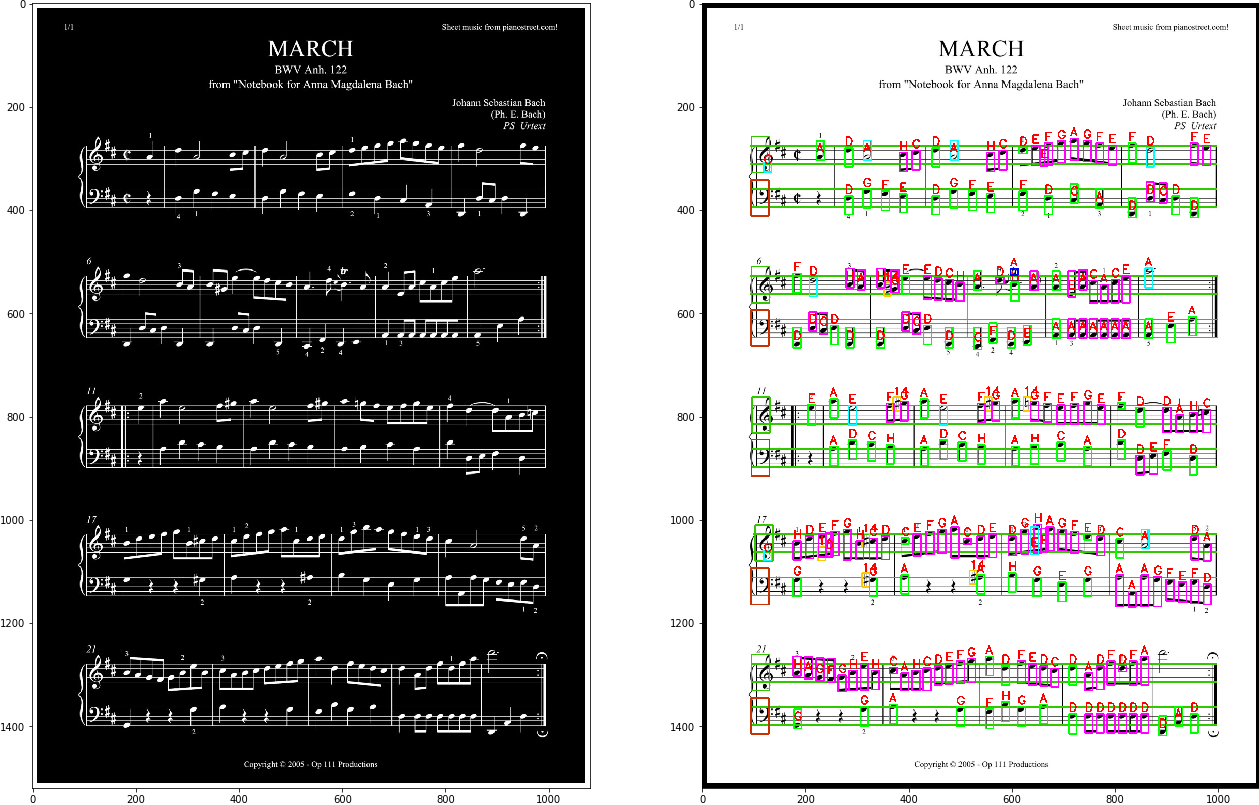
\includegraphics[width=\linewidth]{zdjs/Zdj0.png}
		\caption{Piąty podpis}
	\end{subfigure}
\end{figure}

\section{Podsumowanie, wnioski}
Aplikacja realizuje swój cel, choć są elementy które można by poprawić oraz takie które nie zostały zaimplementowane. Kod zaimplementowany przez nas uzyskuje wysoką skuteczność przy korzystnej scenie zdjęcia; zasadna była by próba ulepszenia kodu poprzez użycie metod adaptatywnych, opartych na funkcji kosztu zamiast metod analitycznych przetwarzania obrazu.

\end{document}
